%
%

%%-----------------------------------------------------
%%-----------------------------------------------------
\section{Servidor web en Producción}

%%-----------------------------------------------------
\begin{frame}
\frametitle{Lo que enseñamos en clase}

\begin{columns}[T]
\begin{column}{.48\textwidth}
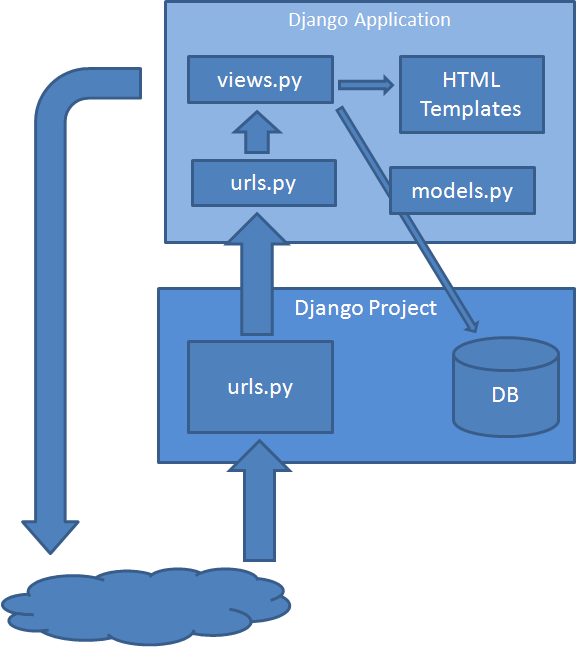
\includegraphics[width=6.5cm]{figs/django}

\begin{flushright}
  {\Large
    \url{http://django-project.com}
  }
\end{flushright}

\end{column}%
\hfill%
\begin{column}{.50\textwidth}
{\Large
\begin{itemize}
  \item Mono-hilo
  \item Mono-tarea
  \item Caché básico
  \item Base de datos limitada (sqlite)
  \item Pensado para páginas dinámicas
  \item Sin planificación
  \item No tiempo real
\end{itemize}
}
\end{column}%
\end{columns}

\end{frame}

%%-----------------------------------------------------
\begin{frame}
\frametitle{Un servidor web en producción}

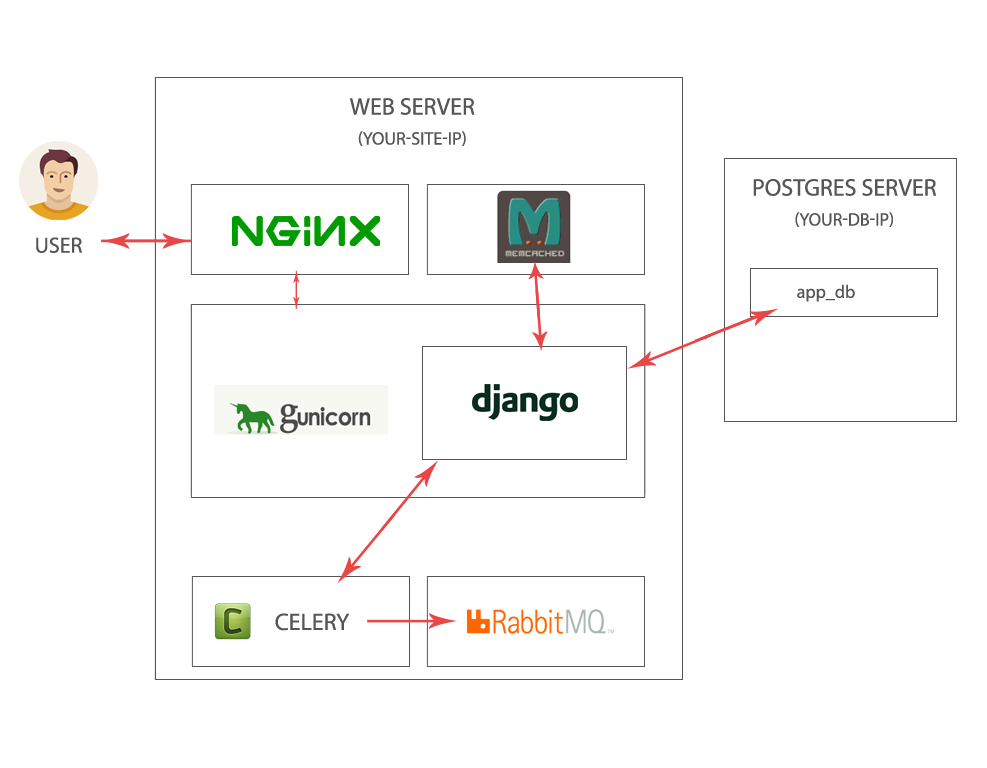
\includegraphics[width=11.5cm]{figs/django-y-mas} 

\end{frame}

%%-----------------------------------------------------
\begin{frame}
\frametitle{Tecnologías}

\begin{itemize}
  \item Django: Framework web
  \item Nginx: Servidor web con balanceo de carga (http://nginx.org/)
  \item Memcached: Caché (http://memcached.org/)
  \item gunicorn: Servidor HTTP (http://gunicorn.org/)
  \item Celery: Tiempo real y planificación de tareas (http://www.celeryproject.org/)
  \item RabbitMQ: Mensajería (https://www.rabbitmq.com/)
  \item PostgreSQL: Base de datos (http://www.postgresql.org/)
\end{itemize}

\end{frame}






